\chapter{複雑系としての社会契約}
本章では、\ref{hypothesis}節で定義した補題3を検証する。
% 「倫理ある商取引ゲーム」において、倫理という限定合理性を仮定した上で商取引システムのインセンティブ設計を行えば、
% プレイヤーの構成によっては不正が防止され、商取引契約の内容が果たされるようになることがわかった。
% 本章では、この商取引契約の内容に焦点を当て、これまで外部の強制執行力として存在が仮定されていた「商取引システム」を、
% ある集団の成員が構成する複雑系の内部で自己組織化されたシステムとして再現する商取引契約の内容について提案し、
% マルチエージェントシミュレーションによって、商取引システムが存在しない場合でも、社会契約が成立しうることを示す。

% \section{本章の問題提起}
% 本章では先の章で扱った「倫理ある商取引ゲーム」において、外部の強制執行力として存在が仮定されていた「商取引システム」が存在しない場合でも、
% プレイヤーの構成によって「商取引ゲーム」の不正を防止することが可能であるかという問いに取り組む。

\section{補題3}
\thirdLemma
% 外部の強制執行力が存在しない場合でも、成員の振る舞いによって強制執行力を自己組織化させることが可能である。

\section{提案手法}
補題1・2の検証で外部の強制執行力として仮定していた「評判システム」を成員達のふるまいとして記述し、
その「評判システム」が検証2の結果と同様の機能を果たすことをマルチエージェントシミュレーションを用いて検証する。
各プレイヤーが「評判システム」を1つずつ所持していると仮定する。
その評判システムの状態を同期させる方法を考える。


\section{分散型評判システム}
各成員が
「評判システム」は、各成員の初期の「評判スコア」と報告された各時刻の約束の記録から現時刻の各成員の「評判スコア」を決定するシステムである。
各成員が「評判システム」を所有している場合、初期の「評判スコア」と各時刻の約束の記録が互いに共有されていれば、
各成員の所有する「評判システム」の現時点の各成員の「評判スコア」は一致する。




\subsection{仮定}
\begin{itemize}
  \item[A1] 送信されたすべてのメッセージは正しく到達する
  \item[A2] メッセージの受信者は誰が送信したのかわかる
  \item[A3] メッセージが届かないことを検知できる
  \item[A4] 誠実な成員の署名は偽造できず、署名されたメッセージの内容が変更されても、それを検知することができる。
  \item[A5] 誰でも成員の署名の信憑性を検証することができる。
\end{itemize}

\subsection{成員の振る舞い}
  \begin{itemize}
    \item 事前の合意に基づいた全ての成員の人数$n$と各成員の初期の「評判スコア」$b_i, ..., b_n$を定義する。
    \item 事前の合意に基づいた全ての成員が互いに$promisor$と$buyer$として1度づつ総当りする周期を定義する。(周期の長さは$ n * (n-1)$)
    \item 事前の合意に基づいた仕様に従った「評判システム」を用意する。
    \item 事前の合意に基づいた商取引契約の内容を定義する。
    \item 各時刻$t$において、「時刻tにおける成員の振る舞い」を上から順に実行する。
  \end{itemize}

\subsubsection{時刻tにおける成員の振る舞い}
\label{behaiverAtTimeT}
\begin{enumerate}
  \item 事前に合意した周期から$promisor$と$reporter$を決定する。
  \item $reporter$は時刻$t-n(n-1)$に$promisor$と交わした約束の結果を決定する。$t \leq n(n-1)$の場合、「成功」とする。
  \item $V_i=\emptyset$として初期化する。($\emptyset$は空集合)
  \item $reporter$は約束の結果を全ての成員に署名して送る。
  \item 各$i$について、 
  \begin{enumerate}
    \item もし$member_i$が$v:0$という形式のメッセージを受け取り、まだ何の報告も受けていない場合は、
    \begin{enumerate}
      \item $member_i$は$ V_i$を${v}$にする。 
      \item $member_i$は他のすべての成員にメッセージ$v:0:i$を送ります。
    \end{enumerate}
    \item もし$member_i$が$v:0:j_1:...:j_k$という形式のメッセージを受け取り、$v$が集合$V_i$に入っていない場合は
    \begin{enumerate}
      \item $member_i$は$v$を$V_i$に追加する。
      \item もし$k<m$であれば、$member_i$は$j_1, ..., j_k$以外のすべての副官に$v:0:j_1:...:j_k:i$というメッセージを送る。
    \end{enumerate}
  \end{enumerate}
  \item 各$i$について、$member_i$がこれ以上メッセージを受け取らない場合、$member_i$は$choice(V_i)$を報告された結果とする。
  \item 各$i$について、$member_i$は報告された結果を自身の「評判システム」に記録する。
  \item $reporter$は$promisor$と新たな約束を交わす。
\end{enumerate}

\section{実験方法}
  ここでは「時刻tにおける成員の振る舞い」のstep 6が必ず遵守される状態を作り出せるかを確認するため、
  下記の「実験用の商取引契約」を合意された商取引契約として、
  これを履行する場合と履行しない場合で4種づつ、計8タイプのエージェントを用意する。
  この8タイプのエージェントから重複問わずランダムに選んだ8体のエージェントを用意し試行を実施する。
  これをタイプAのエージェントが0〜7体を占める場合について、それぞれ8000回づつ繰り返し、
  エージェントの構成とstep9で求まる「報告された成功率」と「真の成功率」を記録する。

  \subsection{実験用の商取引契約}
  $promisor$が「成員の振る舞い」のstep6の通りに振る舞う対価として、$buyer$が通貨を1支払う商取引契約を結ぶ。
  $buyer$は$promisor$がこの商取引を履行したかどうかを「step6の検証」によって確認することができる。

  \subsection{step6の検証}
  時刻$t$において、$buyer$は$promisor$が「成員の振る舞い」のstep6を履行したかを下記の2つの検証で確かめることができる。
  検証1は全てのプレイヤーに同じ商取引の結果を送信したことを検証する方法であり、
  検証2は$buyer$に商取引の結果を送信したかを検証する方法である。
  
  \begin{description}
    % promisorがstep 6で全員に同じ司令を送っていたかの確認
    \item[検証1] 時刻$\max\{0, t-2*n*(n-1)\}$から時刻$\max\{0, t-n*(n-1)\}$までのうち、
      その時刻に行われた商取引の$buyer$が現在時刻の商取引の$promisor$である各時刻$k$について、
      保管されている商取引の記録のうち、時刻が$k$のものを集め、
      その中に報告者が時刻$t$の商取引の$promisor$が存在し、
      それらの結果が一致していることを確認する。
    % promisorがstep 6で自身に司令を送っていたかの確認
    \item[検証2] 時刻$\max\{0, t-2*n*(n-1)\}$から時刻$\max\{0, t-n*(n-1)\}$までのうち、
      その時刻に行われた商取引の$buyer$が現在時刻の商取引の$promisor$である各時刻について、
      保管されている商取引の記録のうち、その時刻の商取引の記録を集めて、
      その中に報告者が現在時刻の商取引の$promisor$である記録が存在するかを確認する。
  \end{description}

  
  \subsection{エージェントの種類}
    下記の8タイプのエージェントを用意する。下記に記述のない振る舞いに関しては「成員の振る舞い」に従う。
    \begin{itemize}
      \item[A] 完全に商取引契約を履行するエージェント
      \item[B] step5を無視して必ず「成功」を報告するエージェント
      \item[C] step5と逆の結果を報告するエージェント
      \item[D] step5を無視して必ず「失敗」を報告するエージェント
      \item[E] step6でタイプAにだけ結果を送らないエージェント
      \item[F] step6でタイプAにだけ結果を送らず、step5を無視して必ず「成功」を報告するエージェント
      \item[G] step6でタイプAにだけ結果を送らず、step5と逆の結果を報告するエージェント
      \item[H] step6でタイプAにだけ結果を送らず、step5を無視して必ず「失敗」を報告するエージェント
    \end{itemize}

  \subsection{試行}
    \begin{description}
      \item[step 1] 時刻tを0とする。
      \item[step 2] 各プレイヤーが互いにpromisorとbuyerのそれぞれの役割で1度づつ商取引ゲームを行う順序を決定し、各エージェントが合意する。(順序の長さは56となる)
      \item[step 3] プレイヤー数は8、初期の通貨保有量は各プレイヤー8、商取引システムの仕様は前章の実験と同じものとし、各エージェントが合意する。
      \item[step 4] 時刻tを1進める。
      \item[step 5] 各エージェントはその特性に則って振る舞う。
      \item[step 6] 各エージェントの「商取引システム」において、時刻tの入力によって誰の通貨保有量も0未満にならない場合、報告された結果を記録する。
      \item[step 7] 各エージェントの「商取引システム」において、時刻tの入力によって誰の通貨保有量も0未満にならない場合、真の結果を記録する。
      \item[step 8] 時刻tが1120未満なら、step4に戻る。
      \item[step 9] 各エージェントの「商取引システム」において、過去56回分のstep5と6で記録された結果を集計し、それぞれ「報告された成功率」と「真の成功率」を求める。
    \end{description}

\section{評価}
% 先の実験の結果、「報告された成功率」と「真の成功率」の両方が100\%になった場合を「不正防止の成功」とし、
% 誠実なエージェント(タイプA)の数と「不正防止の成功」に至った割合をプロットしたものが、図\ref{ethical-game-001}である。
% (エージェント数8の場合は、エージェントの組み合わせが1通りしか存在しないため、個別に試行を行い結果を集計している。)
% 誠実なエージェントの数が0体の場合であっても不正が防止される構成が存在し、
% 6体以上の場合はサンプリングした全ての構成で不正の防止が成功していた。

サンプリングした結果を元に、タイプAのエージェントと自己組織化が成功した割合をプロットすると、
図\ref{compex-system-002}のようになる。この図から、誠実なプレイヤーが6人以上の場合は全てのサンプルで自己組織化に成功していることがわかる。

\begin{figure}[h]
  \begin{tabular}{cc}
    \begin{minipage}[t]{1\hsize}
      \centering
      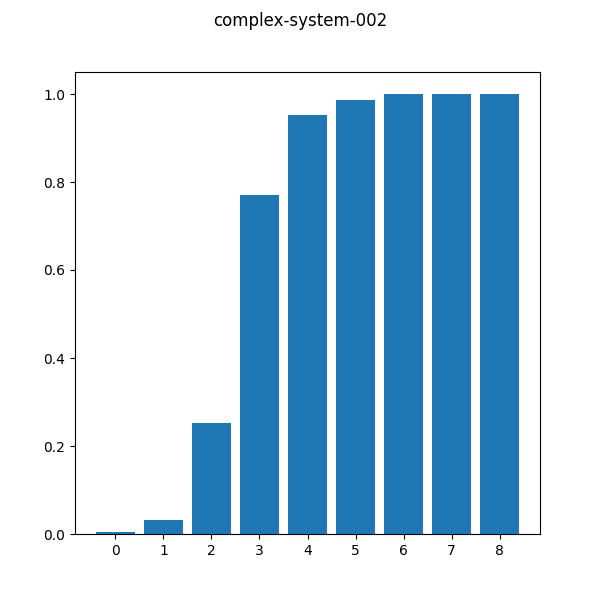
\includegraphics[keepaspectratio, width=1\linewidth]{./07_complex-system/complex-system-002.png}
      \caption{誠実なエージェントの数と自己組織化に成功した割合}
      \label{compex-system-002}
    \end{minipage}
  \end{tabular}
\end{figure}
